\chapter {Performance Analysis}
\label{chap:result}
As we have described the proposed algorithm in the chapter \ref{chap:algorithm}. In this chapter we will discuss about result and performance.
\section{Environments of Experiments}
Text examples in public datasets usually occur within high-quality (high-resolution, well-focused) imagery. In our setting, text often occurs at lower-resolution and with significant blur. Our focus is to achieve text spotting in a real-time system moving through an environment. We first examine how much the information are attached with an analogue image than we detect the text and extract the data. Next, we train the data. Finally, we evaluate the accuracy.
We tested with many different categories of the images such as images are taken with mobile camera, scanning images, DSLR camera and handy cam. The accuracy of the output varied greatly. Accuracy varies mainly for image quality. An image is taken with DSLR camera produce most accurate result. Because of it’s picture quality. Image of DSLR camera is less noise free. So, it’s easy to extract data and OCR can detect the data perfectly. For handy cam images accuracy is slightly get down. Because picture quality is not good as DSLR camera and there is more noise.
If we use scanning images, it produce a good accuracy than handy cam. Because there is less noise than handy cam images. But for mobile camera images the accuracy level is not so good as regarding the other three image categories. For mobile camera there is more noise and image quality is not good.   

\section{Result for English form}
We test our proposed algorithm in different type of sample form. The result depends on the tesseract training data. For english we train "Arial","Courier","Calibri","Times New Roman" fonts. Here we show our some output result and analysis of our training data.
\subsection{Sample form 1}

\begin{figure}[H]
\centering
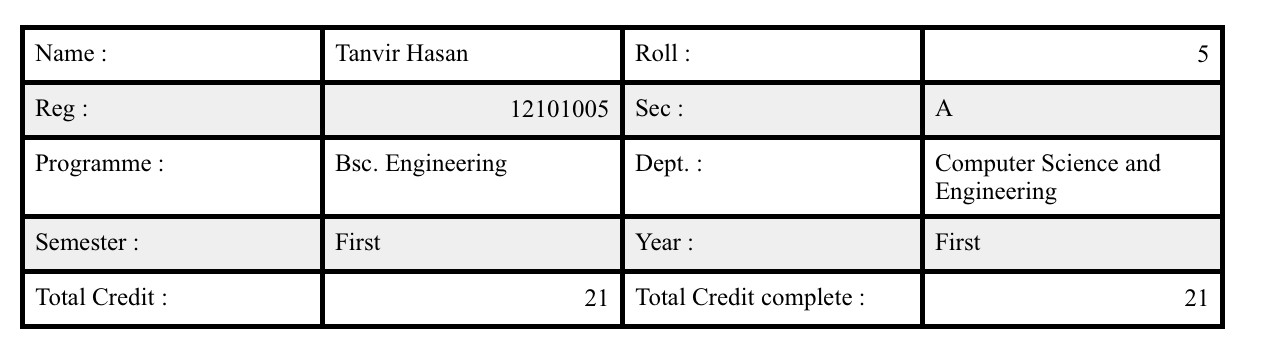
\includegraphics[width=1\textwidth]{form1}
\caption {Sample form 1}
\label {fig:form1}
\end{figure}

\begin{table}[H]
\centering
\begin{tabular}{|p{2cm}|p{2cm}|p{2cm}|}
\hline
character & Input Frequency & Output Frequency \\
\hline
0 & 3  & 3 \\
\hline
1 & 5  & 7 \\
\hline
2 & 3  & 3 \\
\hline
5 & 2  & 2 \\
\hline
8 & 0  & 4 \\
\hline
: & 10 & 10 \\
\hline
A & 1  & 1 \\
\hline
B & 1  & 1 \\
\hline
C & 3  & 3 \\
\hline
D & 1  & 1 \\
\hline
E & 2  & 1 \\
\hline
F & 2  & 2 \\
\hline
G & 1  & 2 \\
\hline
H & 0  & 2 \\
\hline
I & 1  & 1 \\
\hline
N & 1  & 1 \\
\hline
P & 2  & 2 \\
\hline
R & 3  & 3 \\
\hline
S & 3  & 3 \\
\hline
T & 2  & 2 \\
\hline
Y & 9  & 9 \\
\hline
a & 5  & 5 \\
\hline
c & 3  & 3 \\
\hline
d & 18 & 18 \\
\hline
e & 10 & 8 \\
\hline
i & 2  & 1 \\
\hline
l & 6  & 6 \\
\hline
m & 8  & 7 \\
\hline
o & 6  & 6 \\
\hline
p & 3  & 3 \\
\hline
r & 11 & 11 \\
\hline
s & 5  & 5 \\
\hline
t & 10 & 10 \\
\hline
u & 1  & 1 \\
\hline
v & 1  & 1 \\
\hline
\end{tabular}
\caption { Comparison between Input and Output frequency}
\label {tab:Table1}
\end{table}

\begin{figure}[H]
\centering
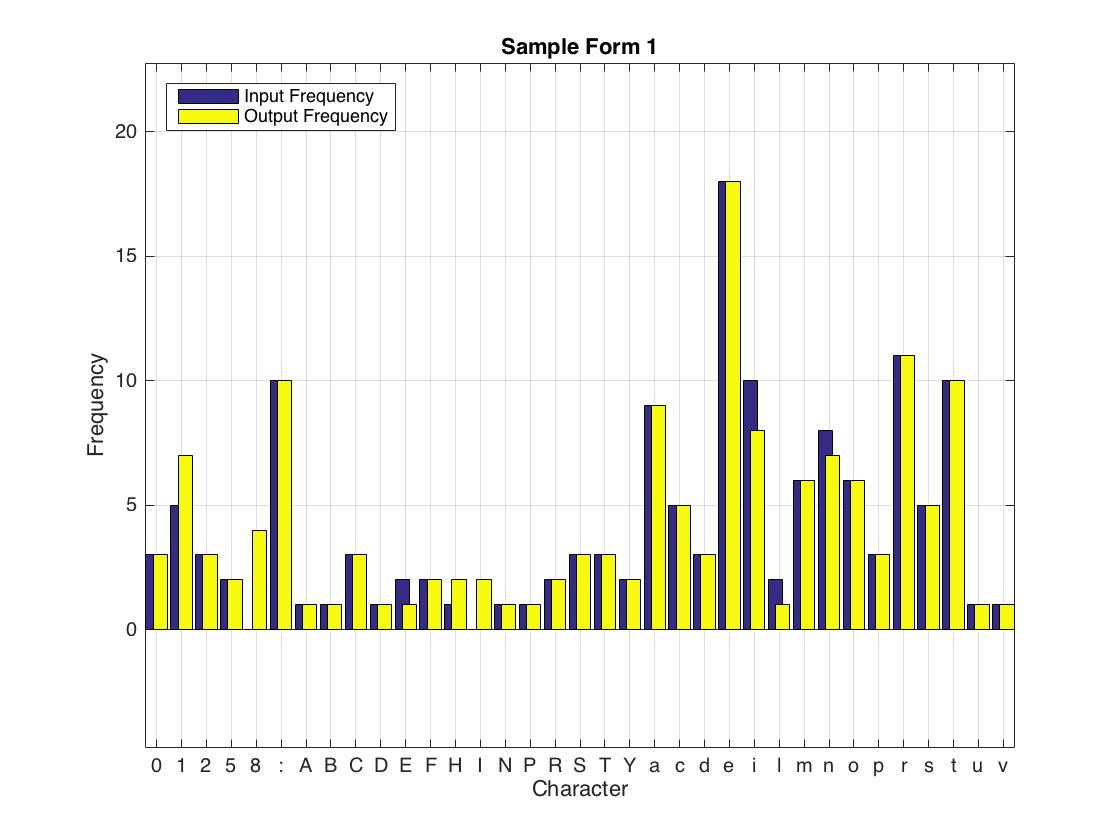
\includegraphics[width=1\textwidth]{Form1}
\caption {Bar chart Input Output Frequency}
\label {fig:bar1}
\end{figure}

\subsection{Sample form 2}

\begin{figure}[H]
\centering
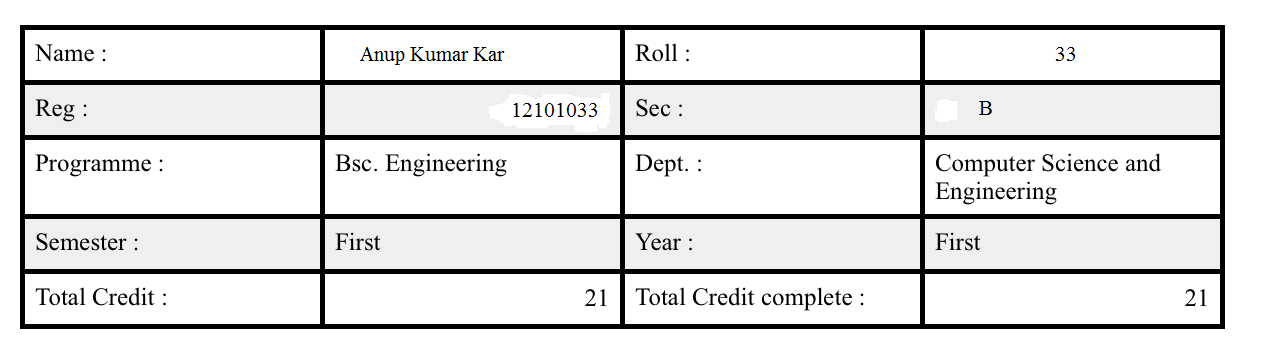
\includegraphics[width=1\textwidth]{form2}
\caption {Sample form 2}
\label {fig:form2}
\end{figure}

\begin{table}[H]
\centering
\begin{tabular}{|p{2cm}|p{2cm}|p{2cm}|}
\hline
character & Input Frequency & Output Frequency \\
\hline
0 & 2 & 1\\
\hline
1 & 5 & 7\\
\hline
2 & 3 & 3\\
\hline
3 & 4 & 4\\
\hline
8 & 0 & 4\\
\hline
: & 10 & 10\\
\hline
A & 1 & 1\\
\hline
B & 2 & 2\\
\hline
C & 3 & 3\\
\hline
D & 1 & 1\\
\hline
E & 2 & 1\\
\hline
F & 2 & 2\\
\hline
H & 0 & 1\\
\hline
I & 0 & 4\\
\hline
K & 2 & 2\\
\hline
N & 1 & 1\\
\hline
O & 0 & 1\\
\hline
P & 1 & 1\\
\hline
R & 2 & 2\\
\hline
S & 1 & 3\\
\hline
T & 2 & 2\\
\hline
Y & 1 & 2\\
\hline
a & 7 & 8\\
\hline
c & 4 & 5\\
\hline
d & 3 & 3\\
\hline
e & 18 & 18\\
\hline
i & 10 & 7\\
\hline
l & 5 & 1\\
\hline
m & 7 & 7\\
\hline
n & 7 & 6\\
\hline
o & 5 & 6\\
\hline
p & 12 & 4\\
\hline
r & 1 & 10\\
\hline
s & 3 & 4\\
\hline
t & 9 & 10\\
\hline
u & 3 & 3\\
\hline
\end{tabular}
\caption {Comparison between Input and Output frequency}
\label {tab:Table2}
\end{table}

\begin{figure}[H]
\centering
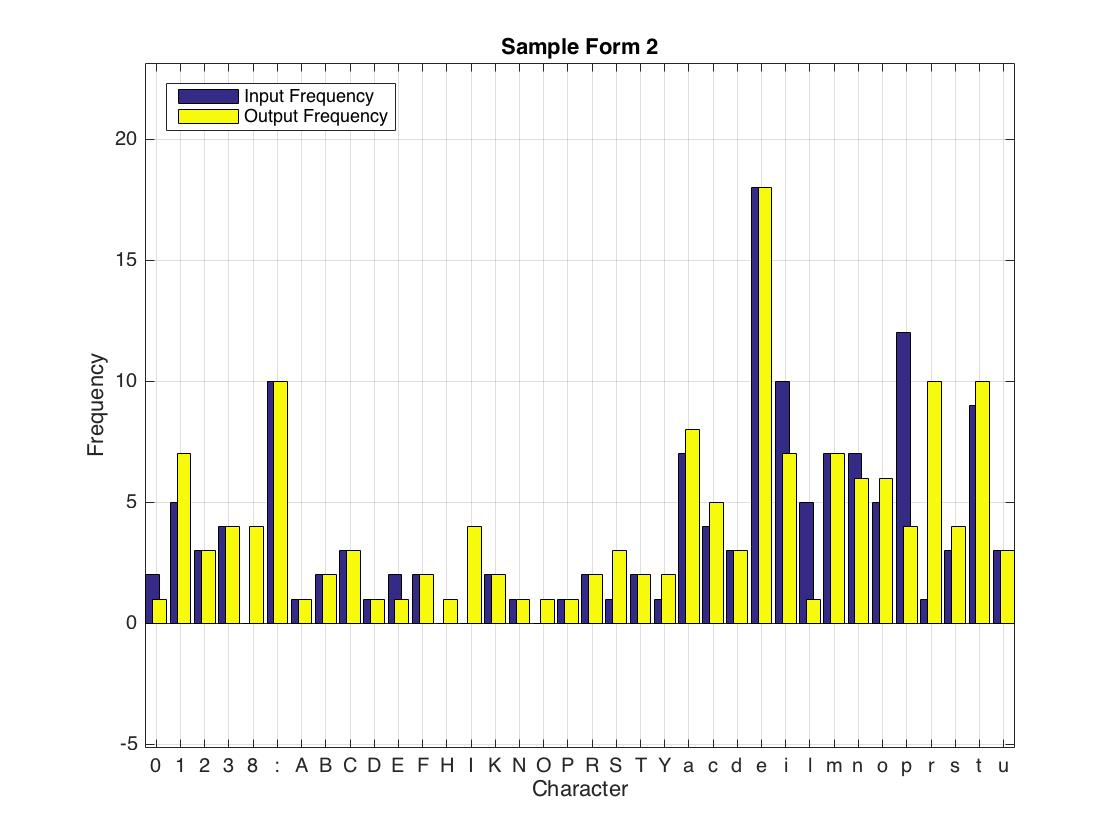
\includegraphics[width=1\textwidth]{Form2}
\caption {Bar chart Input Output Frequency}
\label {fig:bar2}
\end{figure}

\subsection{Sample form 3}

\begin{figure}[H]
\centering
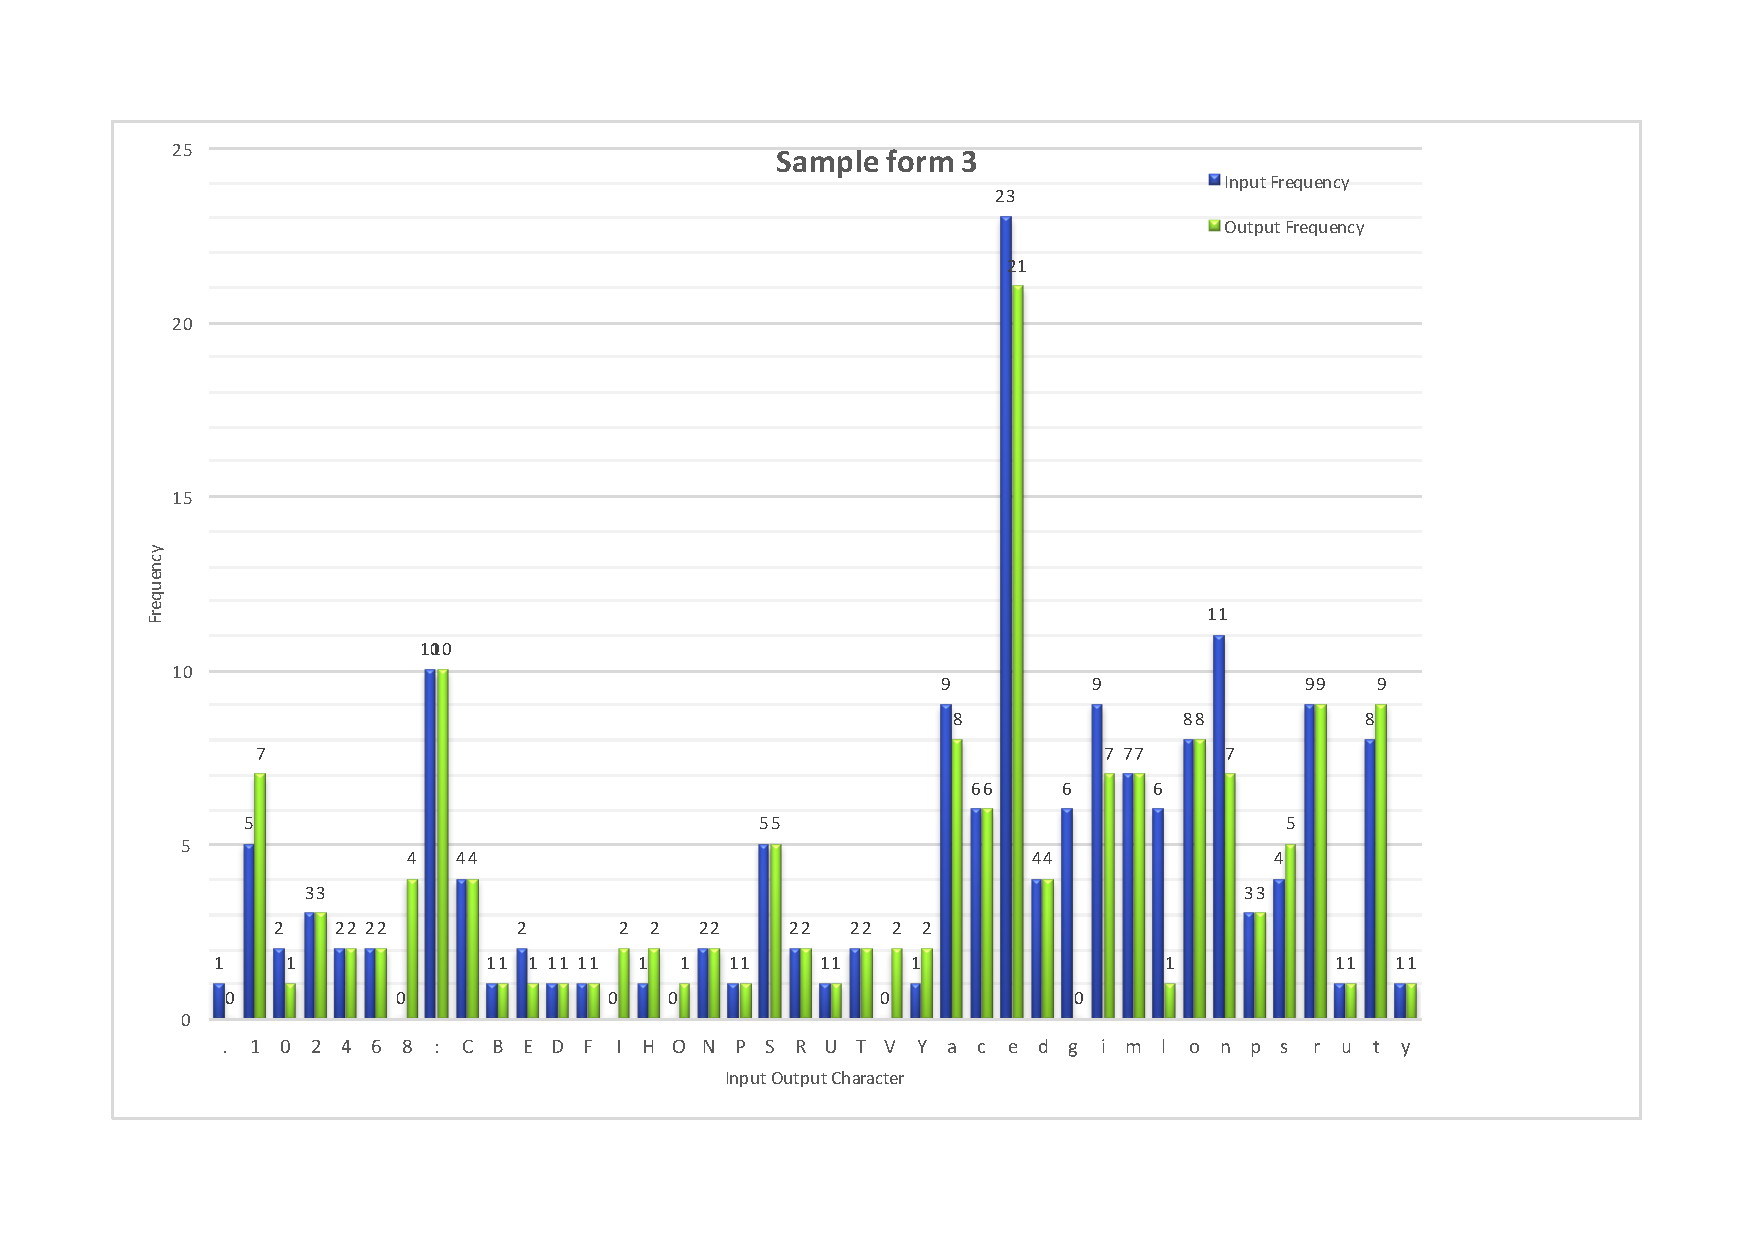
\includegraphics[width=1\textwidth]{form3}
\caption {Sample form 3}
\label {fig:form3}
\end{figure}

\begin{table}[H]
\centering
\begin{tabular}{|p{2cm}|p{2cm}|p{2cm}|}
\hline
character & Input Frequency & Output Frequency \\
\hline
0 & 2 & 1\\
\hline
1 & 5 & 7\\
\hline
2 & 3 & 3\\
\hline
4 & 2 & 2\\ 
\hline
6 & 2 & 2\\
\hline
8 & 0 & 4\\
\hline
: & 10 & 10\\
\hline
B & 1 & 1\\
\hline
C & 4 & 4\\
\hline
D & 1 & 1\\
\hline
E & 2 & 1\\
\hline
F & 1 & 1\\
\hline
H & 1 & 2\\
\hline
I & 0 & 2\\
\hline
N & 2 & 2\\
\hline
O & 0 & 1\\
\hline
P & 1 & 1\\
\hline
R & 2 & 2\\
\hline
S & 5 & 5\\
\hline
T & 2 & 2\\
\hline
U & 1 & 1\\
\hline
V & 0 & 2\\
\hline
Y & 1 & 2\\
\hline
a & 7 & 8\\
\hline
c & 6 & 6\\
\hline
d & 4 & 4\\
\hline
e & 21 & 21\\
\hline
i & 9 & 7\\
\hline
l & 4 & 1\\
\hline
m & 7 & 7\\
\hline
n & 7 & 7\\
\hline
o & 8 & 8\\
\hline
p & 3 & 3\\
\hline
r & 9 & 9\\
\hline
s & 5 & 5\\
\hline
t & 9 & 9\\
\hline
u & 1 & 1\\
\hline
y & 1 & 1\\
\hline
\end{tabular}
\caption {Comparison between Input and Output frequency}
\label {tab:Table3}
\end{table}

\begin{figure}[H]
\centering
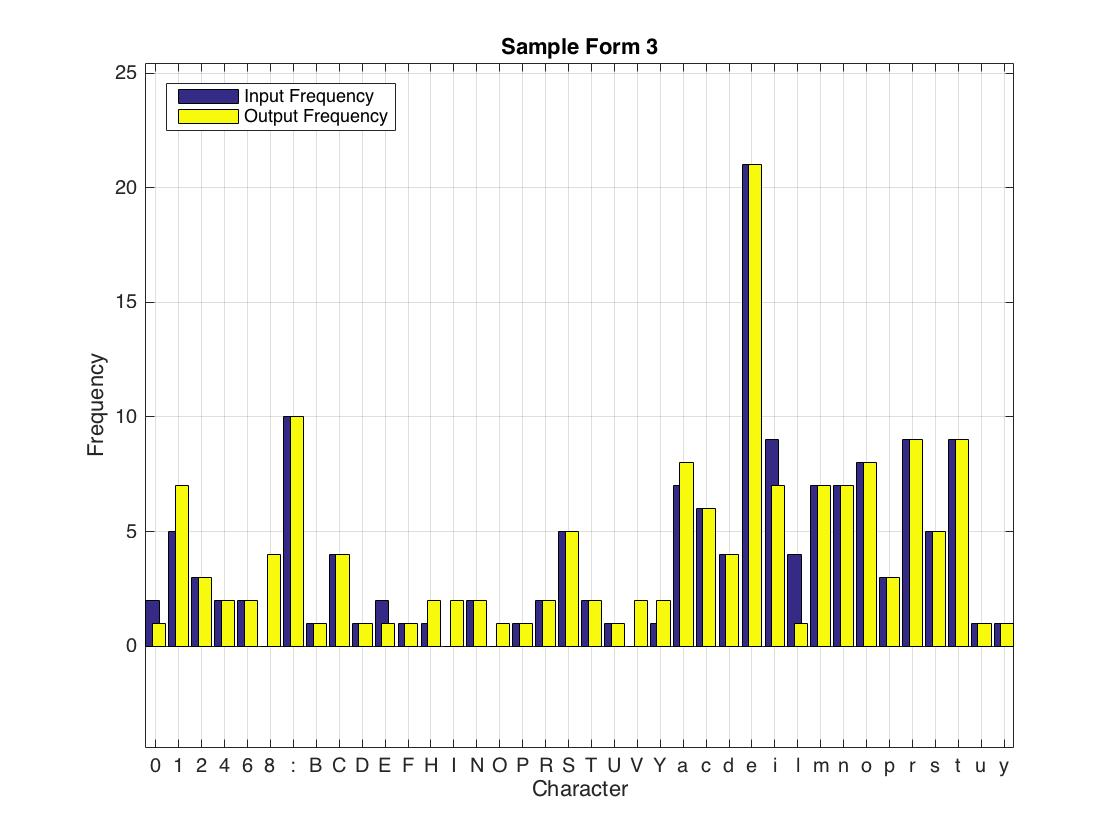
\includegraphics[width=1\textwidth]{Form3}
\caption {Bar chart Input Output Frequency}
\label {fig:bar3}
\end{figure}


\subsection{Sample form 4}

\begin{figure}[H]
\centering
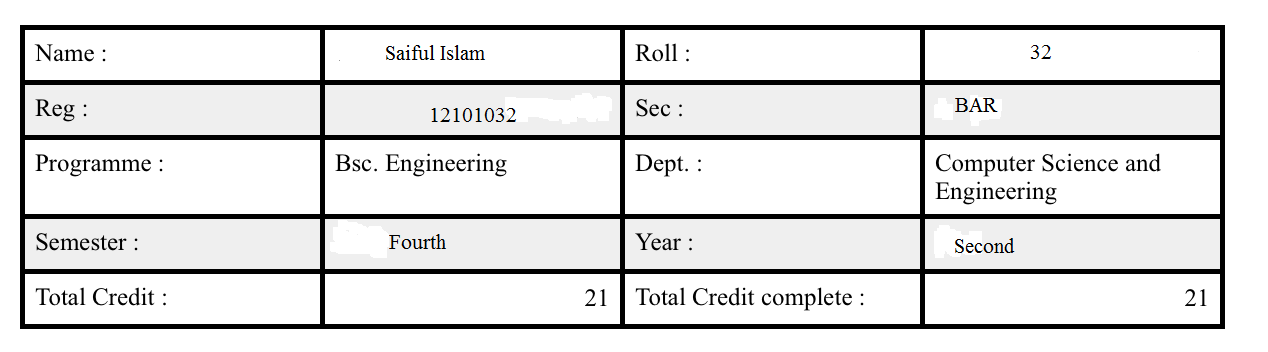
\includegraphics[width=1\textwidth]{form4}
\caption {Sample form 4}
\label {fig:form4}
\end{figure}

\begin{table}[H]
\centering
\begin{tabular}{|p{2cm}|p{2cm}|p{2cm}|}
\hline
character & Input Frequency & Output Frequency \\
\hline
1 & 4  & 10\\
\hline
2 & 5  & 5\\
\hline
3 & 2  & 2\\
\hline
8 & 0  & 4\\
\hline
: & 10 & 10\\
\hline
A & 1  & 1\\
\hline
B & 1  & 2\\
\hline
C & 3  & 3\\
\hline
D & 1  & 1\\
\hline
E & 1  & 1\\
\hline
F & 1  & 1\\
\hline
H & 1  & 1\\
\hline
I & 2  & 2\\
\hline
N & 1  & 1\\
\hline
O & 2  & 2\\
\hline
P & 1  & 1\\
\hline
R & 3  & 3\\
\hline
S & 5  & 5\\
\hline
T & 2  & 2\\
\hline
Y & 2  & 2\\
\hline
a & 8  & 8\\
\hline
b & 1  & 1\\
\hline
c & c  & 6\\
\hline
d & 4  & 4\\
\hline
e & 17 & 19\\
\hline
f & 1  & 1\\
\hline
i & 6  & 6\\
\hline
l & 1  & 1\\
\hline
m & 7  & 7\\
\hline
n & 6  & 6\\
\hline
o & 2  & 8\\
\hline
p & 3  & 3\\
\hline
r & 8  & 8\\
\hline
s & 3  & 3\\
\hline
t & 9  & 10\\
\hline
u & 3  & 3\\
\hline
\end{tabular}
\caption {Comparison between Input and Output frequency}
\label {tab:Table4}
\end{table}

\begin{figure}[H]
\centering
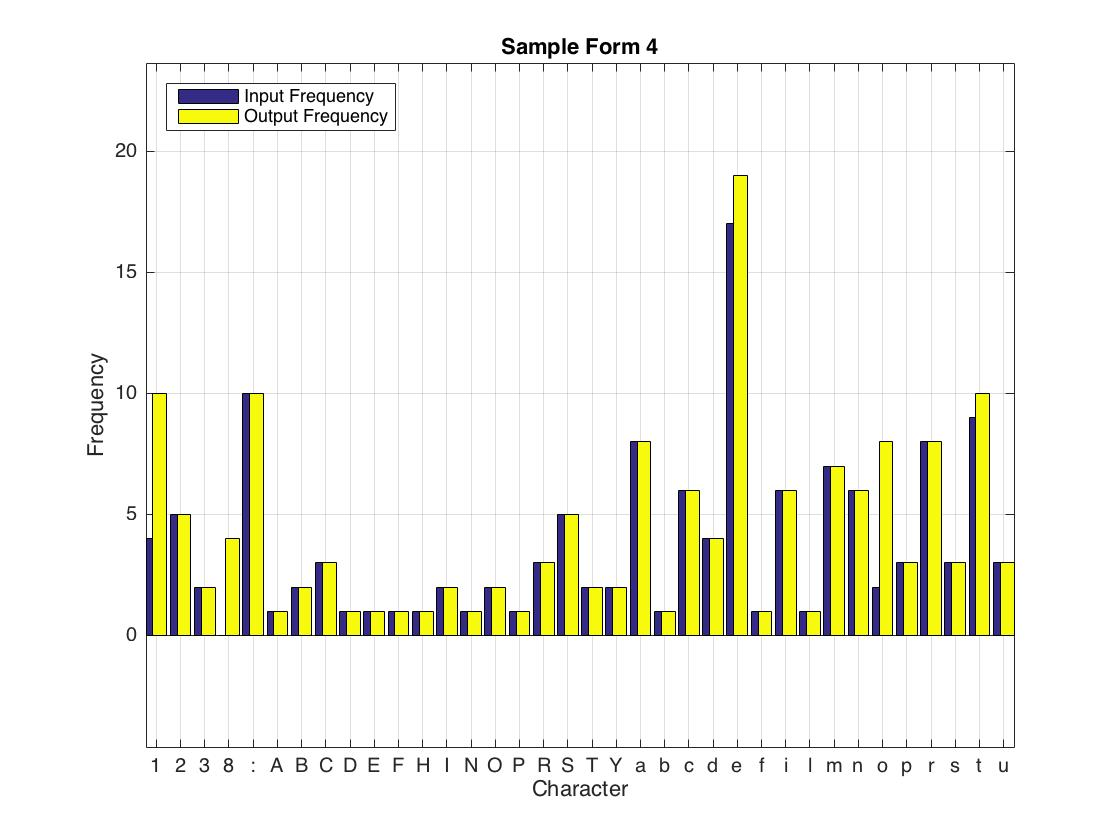
\includegraphics[width=1\textwidth]{Form4}
\caption {Bar chart Input Output Frequency}
\label {fig:bar4}
\end{figure}


\section{Result for Bangla form}
The result of Bangla form depends on the tesseract training data same as English form. For Bangla we train "Siyam rupali" font. Here we show our some output result and analysis of our training data.
\subsection{Sample form 1}
\subsection{Sample form 2}